%----------------------------------------------------------------------------------------
%	INTRODUCTION SLIDES
%----------------------------------------------------------------------------------------

\begin{frame}
\titlepage % Print the title page as the first slide
\end{frame}


\begin{frame} \frametitle{Overview} % Table of contents slide, comment this block out to remove it
\tableofcontents[hideallsubsections] % Throughout your presentation, if you choose to use \section{} and \subsection{} commands, these will automatically be printed on this slide as an overview of your presentation
%\tableofcontents[currentsection]
\end{frame}

%------------------------------------------------
\section{Introduction}
%------------------------------------------------


\begin{frame} \frametitle{Idea}

\begin{block}{Aim}
	Novel work to tackle literature leaks in the scheduling domain applying meteheuristic approaches.
\end{block}

\medskip
\begin{columns}[c]
	\begin{column}[c]{6cm}
		Scheduling domain:
		\begin{itemize}
			\item Energy aware scheduling
			\item Realistic problem (setup, release, due date)
		\end{itemize}
	\end{column}
	\pause
	\begin{column}[c]{6cm}
		Metaheuristic:
		\begin{itemize}
			\item Ant Colony Optimization
			\item Ant Colony System
		\end{itemize}
	\end{column}
\end{columns}

\end{frame}


\begin{frame} \frametitle{Motivation}
\pause
Why scheduling problem?
\begin{itemize}[<+->]
	\item most of daily life problem can easily map in scheduling problem
	\begin{itemize}
		\item industrial/manufacturing environment 
		\item supply-chain management
		\item space orbit 
	\end{itemize}
	\item optimization of shared resources
	\item search for efficiency and cost reduction
	\item avoid critical situation
\end{itemize}

\begin{columns}[c]
	\begin{column}[c]{6cm}
		\begin{figure}
			\centering
			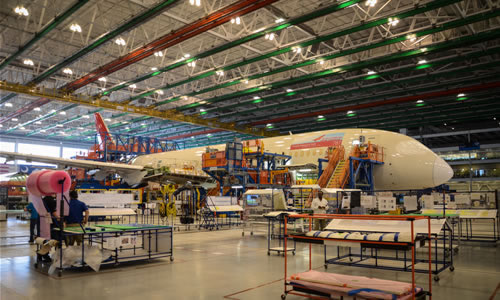
\includegraphics[width=.8\columnwidth]{boeing}
			%\caption{Interaction sequence to solve the distributed scheduling problem}
		\end{figure}
	\end{column}
	\pause
	\begin{column}[c]{6cm}
		\begin{figure}
			\centering
			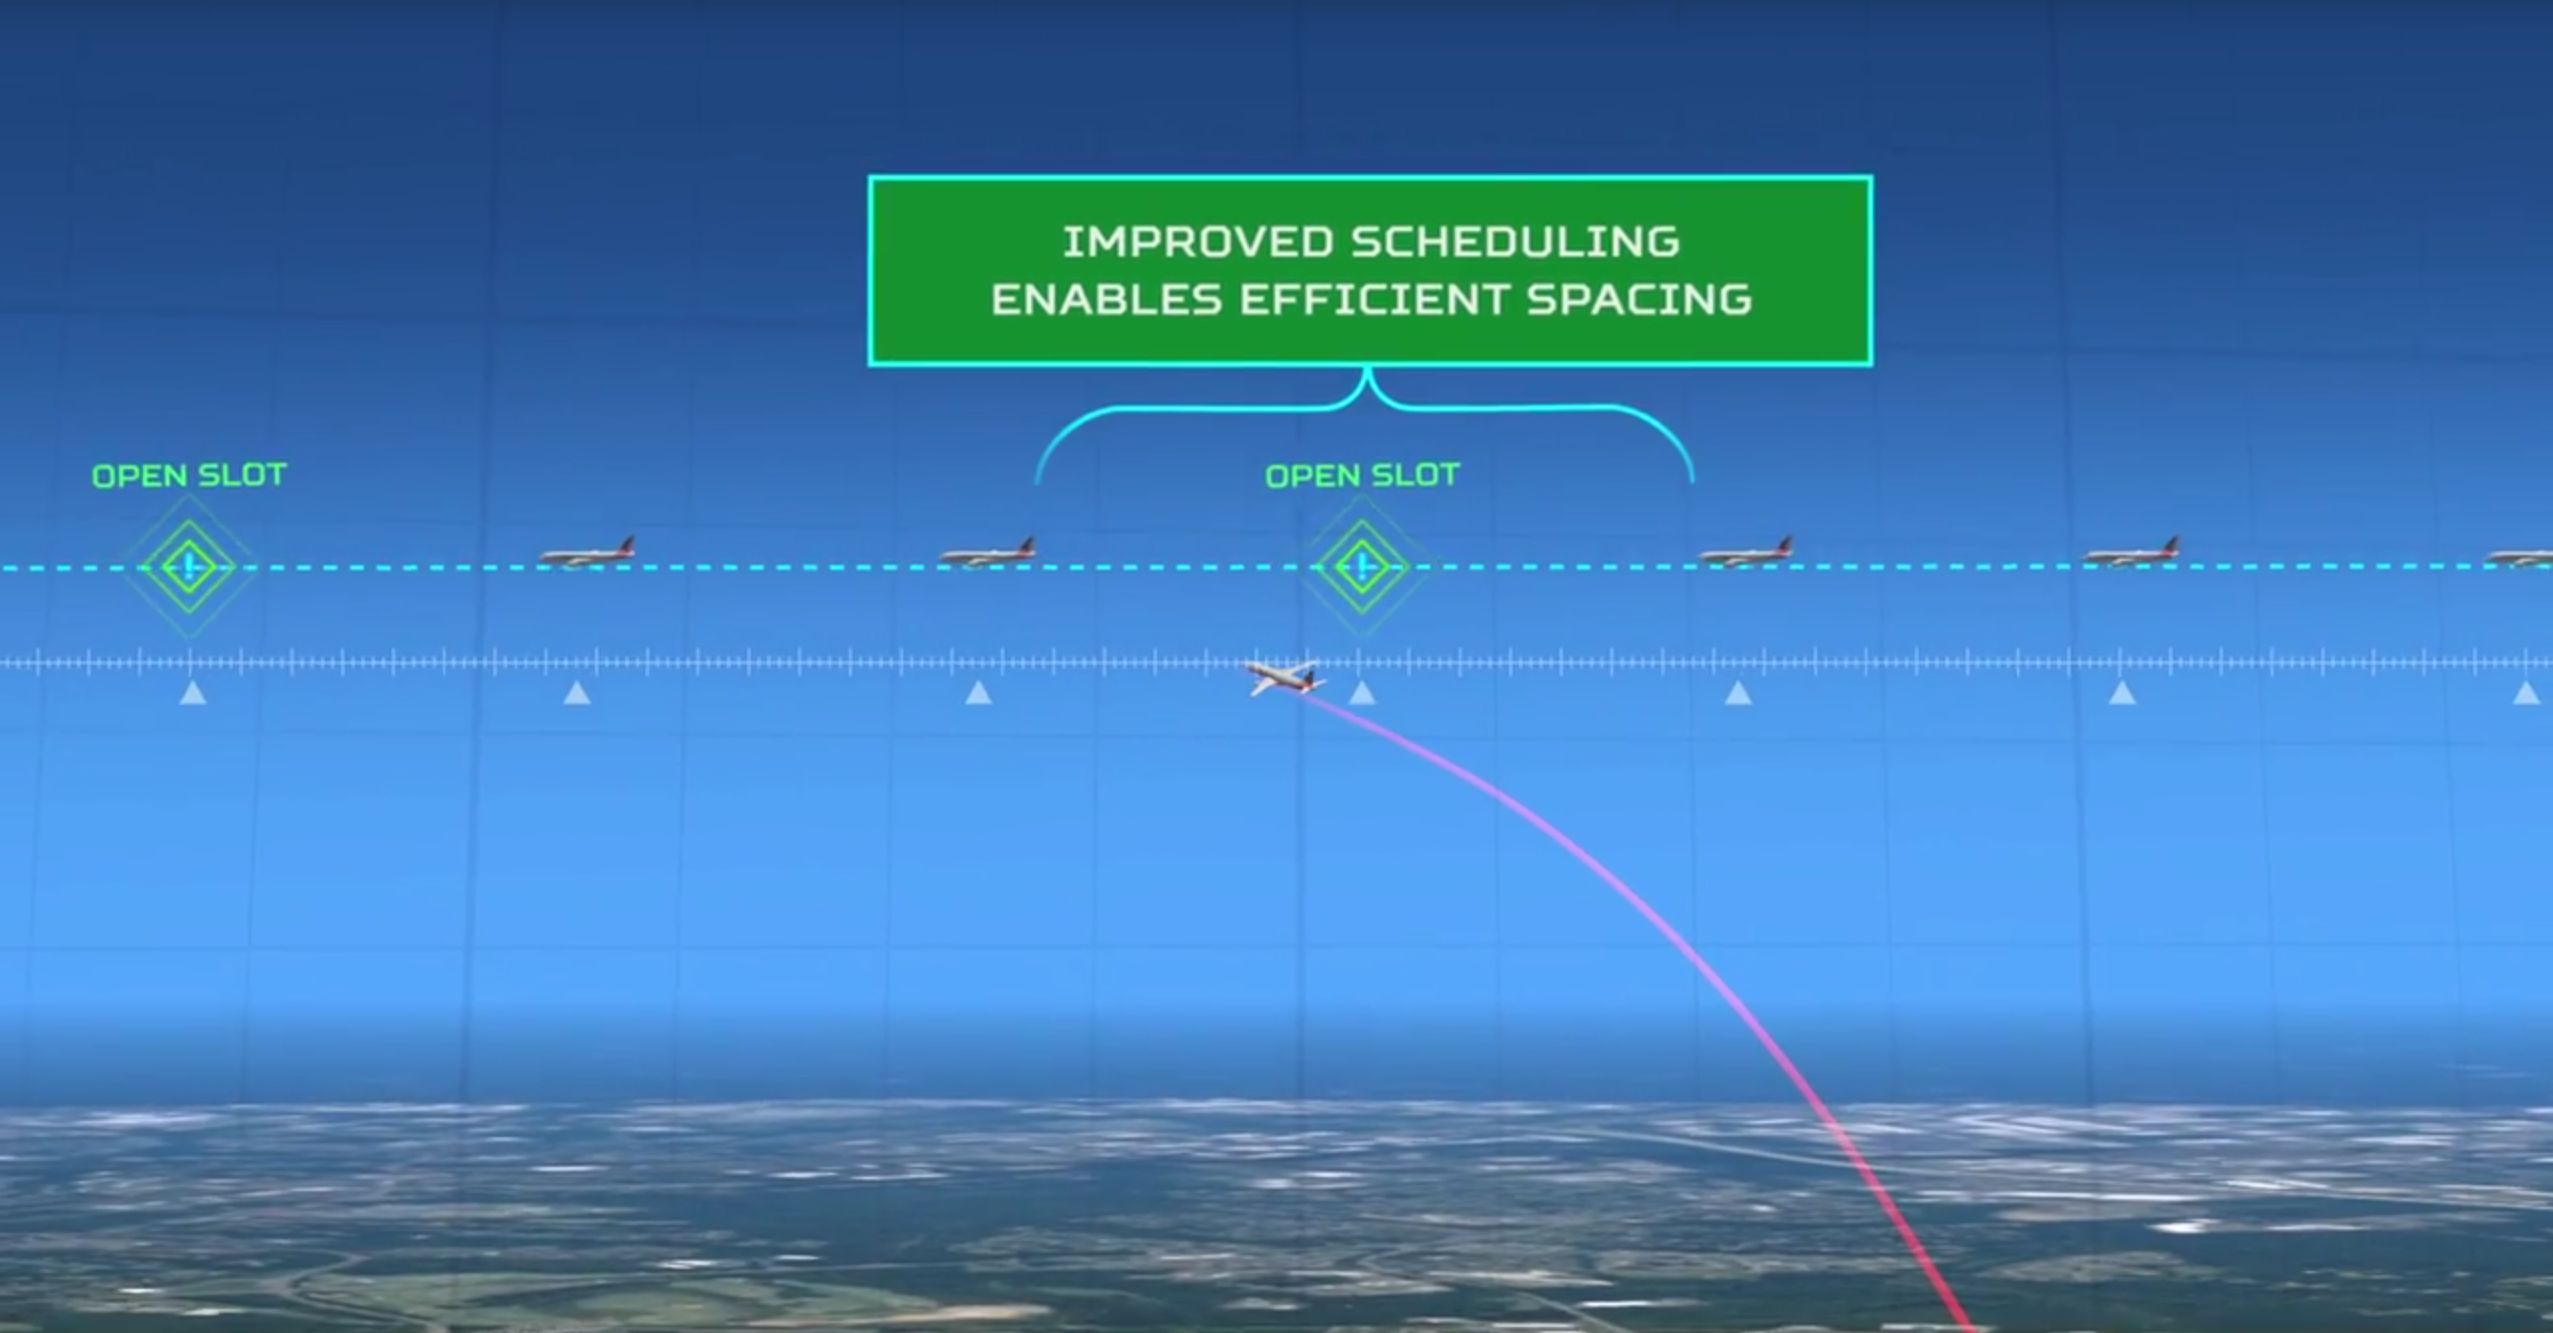
\includegraphics[width=.8\columnwidth]{nasa}
			%\caption{Interaction sequence to solve the distributed scheduling problem}
		\end{figure}
	\end{column}
\end{columns}

\end{frame}